% ****** Start of file apssamp.tex ******
%
%   This file is part of the APS files in the REVTeX 4.2 distribution.
%   Version 4.2a of REVTeX, December 2014
%
%   Copyright (c) 2014 The American Physical Society.
%
%   See the REVTeX 4 README file for restrictions and more information.
%
% TeX'ing this file requires that you have AMS-LaTeX 2.0 installed
% as well as the rest of the prerequisites for REVTeX 4.2
%
% See the REVTeX 4 README file
% It also requires running BibTeX. The commands are as follows:
%
%  1)  latex apssamp.tex
%  2)  bibtex apssamp
%  3)  latex apssamp.tex
%  4)  latex apssamp.tex
%

\documentclass[reprint,amssymb,superscriptaddress,aps,prfluids,onecolumn]{revtex4-2}
\usepackage{amsmath}
\usepackage{array}
\usepackage[usenames,dvipsnames]{color}
\usepackage{epstopdf}
\usepackage{lipsum}
\usepackage{tcolorbox}

\usepackage{graphicx}% Include figure files
\usepackage{dcolumn}% Align table columns on decimal point
\usepackage{bm}% bold math
%\usepackage{hyperref}% add hypertext capabilities
%\usepackage[mathlines]{lineno}% Enable numbering of text and display math
%\linenumbers\relax % Commence numbering lines

%\usepackage[showframe,%Uncomment any one of the following lines to test 
%%scale=0.7, marginratio={1:1, 2:3}, ignoreall,% default settings
%%text={7in,10in},centering,
%%margin=1.5in,
%%total={6.5in,8.75in}, top=1.2in, left=0.9in, includefoot,
%%height=10in,a5paper,hmargin={3cm,0.8in},
%]{geometry}

% --- Make arXiv's pdflatex robust to stray Unicode ---
\usepackage[utf8]{inputenc}   % explicit for older engines in arXiv fleet
\usepackage[T1]{fontenc}

% Map common Unicode you have in the source to TeX math/text
\DeclareUnicodeCharacter{03B8}{\ensuremath{\theta}}   % θ
\DeclareUnicodeCharacter{03C7}{\ensuremath{\chi}}     % χ
\DeclareUnicodeCharacter{2212}{\ensuremath{-}}        % − (minus) → hyphen-minus
\DeclareUnicodeCharacter{2215}{/}                     % ∕ (division slash) → /
\DeclareUnicodeCharacter{2009}{\,}                    % thin space
\DeclareUnicodeCharacter{2011}{\nobreakdash-}         % non-breaking hyphen

% Load hyperref LAST
\usepackage{hyperref}
\hypersetup{
  colorlinks=true,
  urlcolor=blue,
  citecolor=blue,
  linkcolor=black,
  ocgcolorlinks=false  % <-- key: avoid two-layer rendering
}


\begin{document}

\preprint{APS/123-QED}

\title{Supplementary material: \\Holey sheets:Double-Threshold Rupture of Draining Liquid Films}% Force line breaks with \\

\author{Ayush K. Dixit}
\email{a.k.dixit@utwente.nl}
\affiliation{
	Physics of Fluids Department, Max Planck Center Twente for Complex Fluid Dynamics, and J. M. Burgers Center for Fluid Dynamics, University of Twente, P.O. Box 217, 7500AE Enschede, Netherlands
}

\author{Chunheng Zhao}
\email{czhao000@citymail.cuny.edu}
\affiliation{
	Department of Mechanical Engineering, City College of New York, New York, New York 10031, USA
}

\author{St\'ephane Zaleski}
\email{stephane.zaleski@sorbonne-universite.fr}
\affiliation{
	Sorbonne Universit\'e and CNRS, UMR 7190, Institut Jean Le Rond $\partial$'Alembert, 75005 Paris, France
}
\affiliation{
	Institut Universitaire de France, UMR 7190, Institut Jean Le Rond $\partial$'Alembert, 75005 Paris, France
}

\author{Detlef Lohse}
\email{d.lohse@utwente.nl}
\affiliation{
	Physics of Fluids Department, Max Planck Center Twente for Complex Fluid Dynamics, and J. M. Burgers Center for Fluid Dynamics, University of Twente, P.O. Box 217, 7500AE Enschede, Netherlands
}
\affiliation{
	Max Planck Institute for Dynamics and Self-Organisation, Am Fassberg 17, 37077 G{\"o}ttingen, Germany
}

\author{Vatsal Sanjay}
\email{vatsali.sanjay@comphy-lab.org}
\affiliation{CoMPhy Lab, Department of Physics, Durham University, Science Laboratories, South Road, Durham DH1 3LE, United Kingdom}
\affiliation{
	Physics of Fluids Department, Max Planck Center Twente for Complex Fluid Dynamics, and J. M. Burgers Center for Fluid Dynamics, University of Twente, P.O. Box 217, 7500AE Enschede, Netherlands
}



\date{\today}% It is always \today, today,
             %  but any date may be explicitly specified

%\keywords{Suggested keywords}%Use showkeys class option if keyword
                              %display desired
\maketitle

\tableofcontents

\section{Governing equations}\label{sec:gonverning}

The governing dynamical equations have been solved using the free software Basilisk C  \citep{basilliskpopinet, popinet2015quadtree}. For all the quantities, length scales are normalized using the initial bubble radius, resulting in $\mathcal{L} = \tilde{\mathcal{L}}R_0$ as characteristic length, while the time is normalized using the inertiocapillary timescale $\tau_\gamma = \sqrt{\rho_s {R_0}^3/\gamma}$ giving $t = \tilde{t}\tau_{\gamma}$. These normalizations leads to an inertiocapillary velocity scale $u_{\gamma} = \sqrt{\gamma/ \rho_{s} R_0}$ for the velocity field $\boldsymbol{u} = \tilde{\boldsymbol{u}}u_\gamma$. Lastly, stresses are normalized using the Laplace pressure scale, $\boldsymbol{\sigma} = \tilde{\boldsymbol{\sigma}}\sigma_\gamma$, where $\sigma_\gamma = \gamma/R_0$. The governing mass and momentum conservation equations for the liquid phase in dimensionless form read 
\begin{align}
	\label{eq:massconserve}
	\boldsymbol{\nabla\cdot u}=0 \, \text{and}
\end{align}

\begin{equation}
	\frac{\partial \boldsymbol{u}}{\partial t} + \boldsymbol{\nabla\cdot} \left(\boldsymbol{u}\boldsymbol{u}\right) =  -\boldsymbol{\nabla}p + 2\ Oh\boldsymbol{\nabla\cdot}\boldsymbol{\mathcal{D}}, 
	\label{eq:momconserve}
\end{equation}

\noindent where $\boldsymbol{\mathcal{D}} = \left(\boldsymbol{\nabla u} + \left( \boldsymbol{ \nabla u} \right) ^T \right)/2$ represents the symmetric part of the velocity gradient tensor--equal to half of the rate-of-strain tensor, and $p$ is the pressure field. 

\section{Numerical method}\label{sec:methods}
We build upon and employ the open-source software Basilisk C \citep{basilliskpopinet, popinet2015quadtree} to simulate the draining bubbly sheet. The utilized code is shared openly in our repository \cite{coderepository}. The governing equations are solved using the one-fluid approximation \citep{tryggvason2011direct}, with surface tension incorporated as singular body force at the liquid-gas interface \cite{brackbill1992continuum}. To account for the gas phase, we maintain a constant Ohnesorge number based on air viscosity, i.e., $Oh_a = 2 \times 10^{-5}$, and a constant density ratio $\rho_g/\rho = 0.001$. The liquid-gas interface is tracked using the Coupled Level Set volume of fluid (CLSVoF) method. CLSVoF combines some of the advantages of VoF and Level Set (LS) method \cite{sussman2000coupled, basilliskpopinet, saini2025implementation}; this method is mass conserving, which is the advantage of VoF, while the curvature is estimated using the signed distance function, which is the advantage of LS. The interface is tracked using the VoF method governed by the advection equation

\begin{align}
	\frac{\partial \Psi }{\partial t} + \boldsymbol{\nabla\cdot}\left( \Psi \boldsymbol{u}\right) = 0. 
	\label{eq:volfracconserve}
\end{align}

\noindent where $\Psi$ represents the VoF color function. We implement a geometric VoF approach reconstructing the interface at each time step, while the signed distance field $\mathsf{d}$ is advected as a tracer, which is obtained from VoF reconstruction of the interface. The distance is combined with the existing distance using a small weight. Finally,  $\mathsf{d}$ is used to estimate the surface tension forces acting as singular forces \cite{popinet2009accurate, brackbill1992continuum}. The explicit treatment of surface tension imposes a time step constraint based on the smallest capillary wave oscillation period \citep{popinet2009accurate}. 


%\begin{align}
%	\boldsymbol{f}{\gamma} \approx \kappa \boldsymbol{\nabla} \Psi,
%	\label{eq:f}
%\end{align}
%\noindent with curvature $\kappa$ calculated using the height-function method \cite{popinet2018numerical}.

The axisymmetric liquid sheet is simulated in the computational domain spanning $6R_0 \times 6R_0$. A bubble is placed centered on the axis and off the distance $\chi$ from the center of the sheet. At the domain boundaries, velocity conditions are imposed, i.e., $u=\omega \left(6 R_0\right)$ and $v= - 2 \omega \left(6R_0\right)$, while the pressure gradients are set to zero for both liquid and gas phases. The domain is discretized using quadtree grids with adaptive mesh refinement (AMR) \citep{popinet2009accurate}. Error tolerances for the VoF color function, curvature, and velocity are set to $10^{-3}$, $10^{-6}$, and $10^{-3}$, respectively.

\section{Characterize and estimate the initial cavity shape influenced by additional physical inhomogeneities}\label{sec:shape}


As discussed in the main text, in realistic scenarios, chemical or thermal inhomogeneities can delay initial hole nucleation. This delay leads to the formation of a wider thin film region near the poles, which eventually bursts to create a larger cavity. To simulate the initial shape of the sheet with a cavity, we conduct simulations where the interfaces of the bubble and sheet do not coalesce. When the sheet interfaces come into contact with bubble interfaces, instead of merging to create the cavity, sheet interfaces persist on bubble interfaces without coalescence. This is accomplished numerically by introducing different tracers for bubble and surrounding air. The time evolution for non-coalescing simulations is shown in fig. \ref{fig:ab_time}. At any time $t_r$, the thin bridge region is manually ruptured to obtain the cavities characterized by $\theta$ -- large $t_r$ corresponds to wider cavities, and thus, large $\theta$. Therefore, for simulations to assess the effect of different initial cavities, the initial condition is taken as the profile at time $t_r$ after removing the thin film cap. This approach has been widely adopted in numerous studies related to floating bubbles \cite{duchemin2002jet, deike2018dynamics}. 

The initial cavity profile is characterized by the angle $\theta (Bo, t_r)$, which is obtained by selecting the parameters $Bo$, and $t_r$. However, remarkably, the shape is observed to be the same, regardless of $Bo$, and $t_r$ as long as $\sqrt{Bo} \times t_r$ is same. Thus, the initial cavity shape $\theta(\sqrt{Bo} \ t_r)$ is observed to be solely determined by $\sqrt{Bo} \times t_r$ for $Bo < 10^{-2}$ which includes almost all the realistic scenarios. For higher $Bo > 10^{-2}$, unlike small $Bo$ cases, the minimum bubble-sheet thickness is no longer at the poles; instead, a small liquid volume is sandwiched at the poles, and the minimum thickness is observed off the poles. This observation poses a resemblance with the drop impact phenomenon \cite{bouwhuis2012maximal}, where for small Stokes number $St$, no air bubble is entrapped below the droplet. Also, the minimum thickness of the drop-plate interface is at the poles--similar behavior is observed here for $Bo < 10^{-2}$. In contrast, for larger $St$, air bubbles are entrapped, and the minimum thickness is observed away from the poles, which is similar to behavior here at larger $Bo > 10^{-2}$. 

\begin{figure}[h!]
	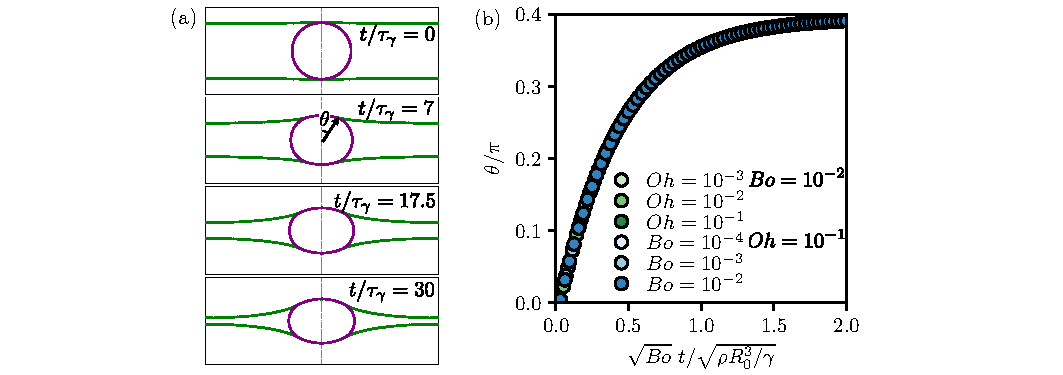
\includegraphics{ab-time_02.pdf}
	\caption{\label{fig:ab_time}  (a) The time evolution of the draining sheet when the bubble-sheet interfaces do not coalesce at $Oh=0.1$, and $Bo=10^{-3}$. The green and magenta depict the sheet and bubble interfaces, respectively. The shape is characterized by the angle $\theta$, which is the circumferential angle covered by the overlapping bubble-sheet interfaces. (b) The evolution of $\theta$ against $ \sqrt{Bo} \ t_r/\sqrt{\rho R_0^3/\gamma}$ for various $Bo$ and $Oh$ higlights that the shape evolves independently of $Bo$ and $Oh$ and is solely determined by $ \sqrt{Bo} \ t_r/\sqrt{\rho R_0^3/\gamma}$. 
	}
\end{figure}
 
 \section{Effects of bubble asymmetry $\chi/R_0$}\label{sec:asymmetry}
When the bubbles are placed asymmetrically in axial direction ($\chi/R_0 > 0$), the sheet no longer ruptures immediately, and the presence of the intact liquid bridge reduces the tendency of the sheet to break compared to the corresponding symmetric case, which is the least stable one. 
In the asymmetric cases illustrated in fig. \ref{fig:OhBo-chi}, the darker zones depict the regions where the effect of the initial bubble on bubble breakup is still prominent. These regions are narrower compared to the opening regime of symmetric cases at the right side of the gray transition line, bolstering the fact that the addition of asymmetricity reduces the tendency of sheets to break. As $\chi/R_0$ increases, the effect of the asymmetry becomes even more pronounced. That is, the tendency of the sheets to break reduces even further. This aspect is also evident in fig. \ref{fig:OhBo-chi} where the lighter yellow regions enlarge, while the darker zones shrink as one increases $\chi/R_0$ from $0.05$ to $0.15$. 

\begin{figure}[h!]
	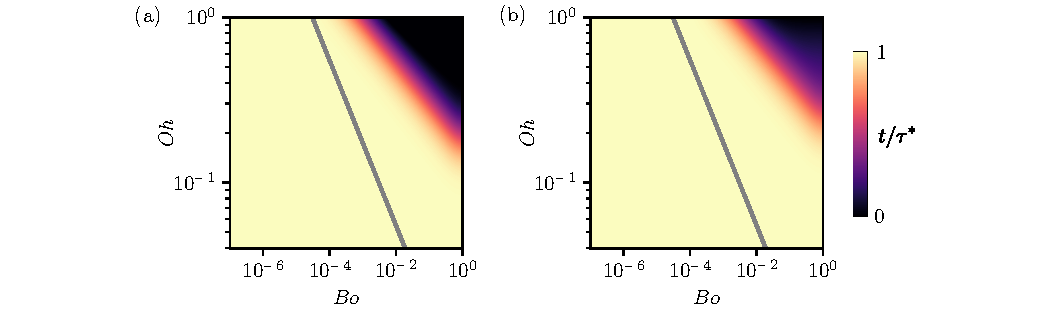
\includegraphics{OhBo-chi_01.pdf}
	\caption{\label{fig:OhBo-chi}  Sheet breakup time (normalized by the no-bubble case rupture time $\tau^* \sim \tau_\gamma/\sqrt{Bo}$) in the $Oh-Bo$ parameter space, at (a) $\chi/R_0 = 0.05$, and (b) $\chi/R_0 = 0.15$. The gray line depicts the transition observed for symmetric cases ($\chi/R_0 = 0$). 
	}
\end{figure}

%\section{Supplementary movies' captions}\label{sec:supplementary}

%\nocite{*}
\bibliographystyle{prsty_withtitle}
\bibliography{holeySheets}% Produces the bibliography via BibTeX.

\end{document}
%
% ****** End of file apssamp.tex ******
